\documentclass[10pt]{book}
\usepackage{cdt/cdtAnalisis}
\usepackage{tikz}
%%%%%%%%%%%%%%%%%%%%%%%%%%%%%%%%%%%%%%%%%%%%%%%%%%%%%%%%%%%%%%%%
% Datos del proyecto

\cdtOrganizacion[CBR]{Club de Bio-Robóticoa de ESCOM}

\cdtAutor{Coordinación de Desarrollo Tecnológico, IPN}

\cdtSistema[PAG]{Página del Club de Bio-Robótica}

\cdtProyecto[RED]{Rediseño de la página}

\cdtDocumento{PT}{Propuesta técnica}{\DRAFT{\today}} %\RELEASE{1.0}

\cdtEntregable{E1}{Entregable 1}

% Descomentar y establecer la fecha cuando se desee congelar la fecha del documento.
%\cdtFecha{12 de Abril de 2013}

%%%%%%%%%%%%%%%%%%%%%%%%%%%%%%%%%%%%%%%%%%%%%%%%%%%%%%%%%%%%%%%%

\begin{document}

%=========================================================
% Portada
\thispagestyle{empty}

\maketitle

%=========================================================
% Indices del documento
\frontmatter
\tableofcontents
\listoffigures
\listoftables
\mainmatter

% Para esconder la información del documentador se descomenta el \hideControlVersion
%\cdtHideControlVersion
%\cdtHideInstrucciones


%=========================================================

En este documento se presentará el análisis, diseño, construcción y las pruebas de nuestro Sistema Administrador de Clínicas, así como la metodología usada y las etapas que harán que el sistema vaya creciendo y permita resolver las problemáticas que actualmente enfrenta la empresa.

El presente documento se encuentra divido por 7 bloques: Introducción, Análisis de problema, Propuesta de solución, Modelo de Negocios, Modelo de despliegue del sistema, Modelo de comportamiento y modelo de la iteración.

En la introducción que en este momento lee se da una pequeña reseña del trabajo, así como los acrónimos, abreviaturas y referencias bibliográficas que se han consultado con el fin de diseñar este documento de la forma más amigable y entendible para el lector.
En la sección de Análisis del problema se tratará el contexto del sistema, el cual define cómo se mueve la empresa actualmente; los procesos actuales, que describe quiénes y cuál es su puesto dentro del sistema; los problema identificados, que son las razones que lleva a la empresa a solicitar un sistema y que no permiten que funcione de manera eficaz; y, finalmente, las propuestas de solución, que son las alternativas que se podrían aplicar para resolver los problemas identificados, de esas alternativas de solución se seleccionará la que mejor resuelva el problema y cumpla los requisitos que la empresa solicita.

La propuesta de solución se desglosará planteando primeramente los objetivos: un objetivo general y varios partículares, que serán las metas que queremos lograr con nuestro sistema; y se tratará el modelo de despliegue abarcando los requerimientos no funcionales, el modelado de dicho despliegue y las especificaciones de la plataforma.

El modelo de negocios nos permitirá definir cómo trabaja la empresa actualmente y si en algún punto el software que se planea implementar podría llegar a cambiar la forma en la que se mueve la empresa. Primeramente se creará un glosario de términos para entender la jerga de los empleados, se tratarán los procesos ajustados, así como los procesos actuales, la descripción de atributos y finalmente las reglas del negocio, que son las principales y son las que rigen todo sistema.

El modelo de despliegue del sistema en una sección encargada de mostrar cómo nuestro sistema se va desarrollando a través del tiempo y cómo está estructurado.

El modelo de comportamiento describe qué funcionalidades tiene el sistema y cómo debe reaccionar ante diversos eventos que genere el usuario, describiendo sus atributos y cómo se va a mover el sistema en caso de entradas no esperadas.

El modelo de iteraciones presentará la descripción completa de la sinterfaces de usuario y cómo éste puede manipularlas e interactuar con ellas para obtener un resultado definido.

Este documento va dirigido al profesor Ulises Vélez Saldaña, profesor de la Escuela Superior de Cómputo del Instituto Politécnico Nacional como un proyecto de desarrollo de software.

Este documento será realizado por 'The Dream Team', conformado por:

- Martínez Vilchis Juan Moisés.

- Moreno González Gabriela.

- Pérez Montiel Ulises.

- Reynoso Rodríguez Erick Rubén.

Realizado en la Escuela Superior de Cómputo del Instituto Politécnico Nacional, mediante una organización secuencial de las partes que se irán cubriendo del documento y de la presentación final.

%--------------------------------------------------
\section{Alcance}
Nuestro proyecto planea cubrir todos los requerimientos funcionales y no funcionales que serán planteados y analizados a lo largo del proyecto para resolver las problemáticas principales. Se espera que los problemas secundarios sean tratados en tiempo posterior a la entrega de este proyecto.

%--------------------------------------------------
\section{Notaciones, estándares y UML.}

\begin{description}
	\item[Servidor:] Como el manejo será local, un servidor se entiende como el software que configura un PC como servidor para facilitar el acceso a la red y sus recursos.
\end{description}

\begin{description}
	\item[UML:] Unified Modeling Language (Lenguaje de Modelado Unificado), es un lenguaje estándar utilizado para modelar diagramas de clases, de secuencias, etc.
\end{description}

\begin{description}
	\item[Scrum:] Es una metodología de desarrollo de software.
\end{description}

\begin{description}
	\item[Diagrama de Ishiwaka:] Son diagramas empleados para profundizar de una manera gráfica al menos 6 aspectos dentro de una problemática global.
\end{description}

\begin{description}
	\item[Requerimientos funcionales:] Son todas aquellas acciones que requiere hacer el sistema y que necesita el usuario.
\end{description}

\begin{description}
	\item[requerimientos no funcionales:] Son todas aquellas acciones o aspectos que deben cumplir las acciones que se realizan 'detrás' de los requerimientos funcionales para su correcta implementación.
\end{description}

\begin{description}
	\item[Business Motivation Model:] Provee un esquema o estructura para desarrollar, comunicar, y gestionar los planes de negocio de una manera organizada.
\end{description}

\begin{description}
	\item[Business Process Modeling Notation:] Es una notación utlizada para modelar procesos dentro de una empresa mediante el conocimiento de las reglas del negocio y de los procesos actuales.
\end{description}

\begin{description}
	\item[Caso de uso:] Es una descriptiva de una acción que debe realizar el sistema, especificando los valores de entrada, las salidas y las pantallas en las que se llevará a cabo dicha acción.
\end{description}

\begin{description}
	\item[Botón:] Es un componente de java swing que permite la realización de determinadas acciones al presionarse.
\end{description}

\begin{description}
	\item[Campo de texto:] Es un componente de java swing que permite al usuario ingresar una cadena de texto.
\end{description}

\begin{description}
	\item[Reglas del negocio:] Son todas aquellas sentencias que definen la operación del negocio y permiten a los participantes tomar decisiones.
\end{description}

\begin{description}
	\item[Package:] Es una agrupación de clases afines.
\end{description}

\begin{description}
	\item[Diagrama de despliegue:] Son los diagramas que muestran las clases que contiene un package.
\end{description}

%=========================================================
\documentclass[oneside,10pt]{book}

\usepackage{cdtBook}
\usepackage{usecases}

\title{SCVME}
\subtitle{Sistema de Compra y Venta de Material Electrónico}
\author{Sworkware}
%\organization{Escuela Superior de Cómputo, IPN}


%%%%%%%%%%%%%%%%%%%%%%%%%%%%%%%%%%%%%%%%%%%%%%%%%%%%%%%%%%%%%%%%
\begin{document}

\maketitle
\thispagestyle{empty}

\frontmatter
\tableofcontents

\mainmatter

%=========================================================
\chapter{Introducción}

\cfinput{introduccion}

%=========================================================
\chapter{Análisis del problema}

\cfinput{problematica}

%=========================================================
\chapter{Propuesta de solución}

\cfinput{propuesta}



%=========================================================
\chapter{Modelo de Negocios}

\cfinput{brGlosario}
\cfinput{brProceso}
\cfinput{brModelo}
\cfinput{brReglas}

%=========================================================
\chapter{Modelo del despliegue del sistema}

%=========================================================
\chapter{Modelo de comportamiento}
	
	\begin{figure}[htbp!]
		\centering
			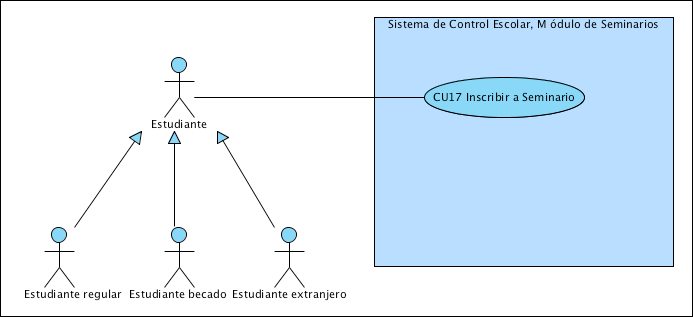
\includegraphics[width=0.8\textwidth]{images/CasosDeUso}
		\caption{Diagrama de Casos de Uso del sistema.}
	\end{figure}
	
	\begin{figure}[htbp!]
		\centering
			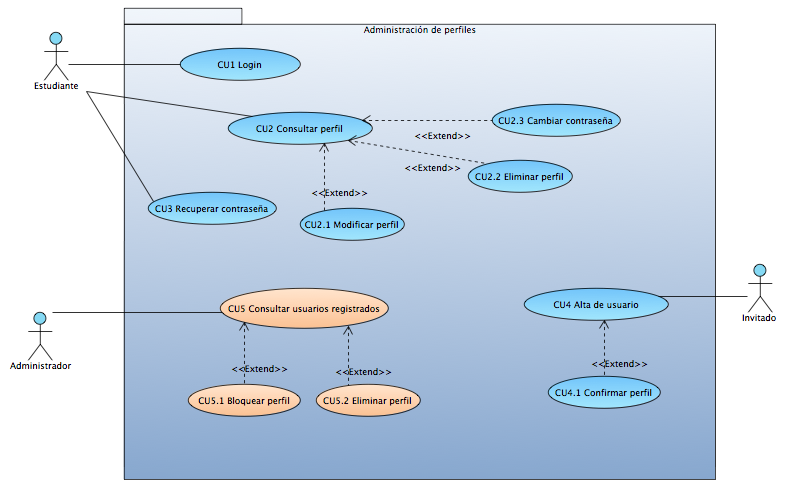
\includegraphics[width=0.8\textwidth]{images/CasosDeUso1}
		\caption{Diagrama de Casos de Uso del sistema.}
	\end{figure}
	
	\begin{figure}[htbp!]
		\centering
			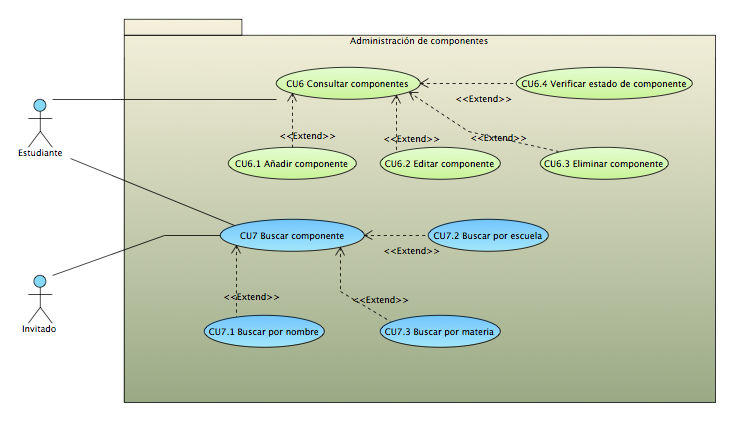
\includegraphics[width=0.8\textwidth]{images/CasosDeUso2}
		\caption{Diagrama de Casos de Uso del sistema.}
	\end{figure}
	
	\begin{figure}[htbp!]
		\centering
			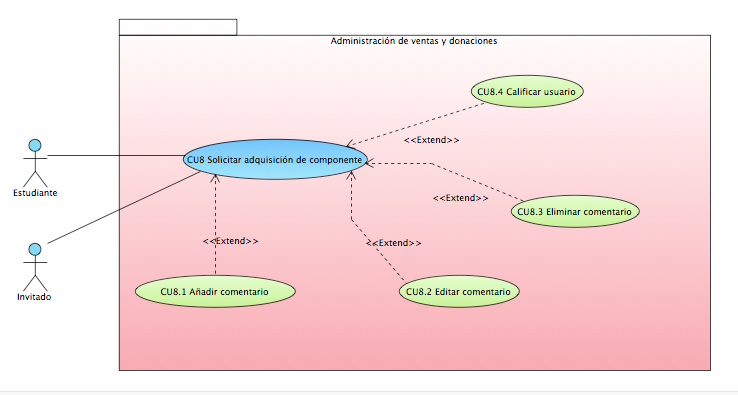
\includegraphics[width=0.8\textwidth]{images/CasosDeUso3}
		\caption{Diagrama de Casos de Uso del sistema.}
	\end{figure}
	
	\begin{figure}[htbp!]
		\centering
			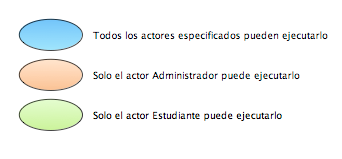
\includegraphics[width=0.8\textwidth]{images/CasosDeUso4}
		\caption{Diagrama de Casos de Uso del sistema.}
	\end{figure}
	
	\begin{figure}[htbp!]
		\centering
			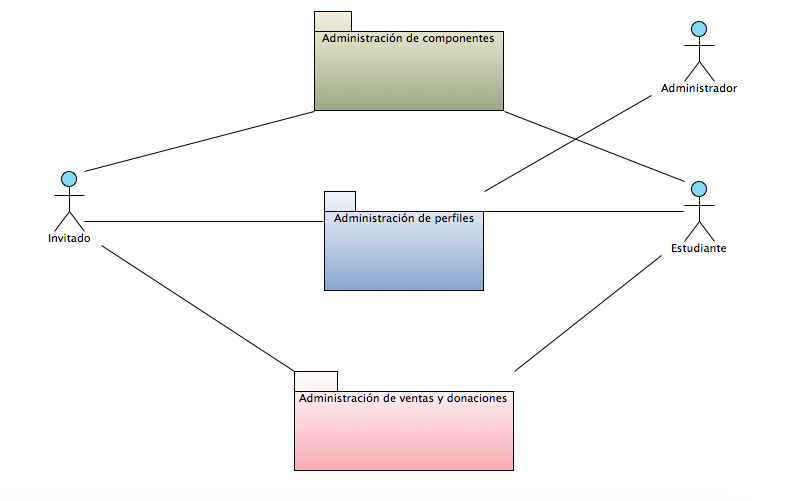
\includegraphics[width=1\textwidth]{images/CasosDeUso5}
		\caption{Diagrama de Casos de Uso del sistema.}
	\end{figure}
	
\cfinput{cu/cu12}
\cfinput{cu/cu13}
%\cfinput{cu1/cu}
%\cfinput{cu2/cu}
%\cfinput{cu3/cu}
%\cfinput{cu4/cu}
%\cfinput{cu5/cu}

%%=========================================================
\chapter{Modelo de la Interacción}

%\cfinput{Pantallas/navegacion}

\cfinput{Pantallas/IU5}
%\cfinput{Pantallas/IU1}
%\cfinput{Pantallas/IU2}
%\cfinput{Pantallas/IU3}
%\cfinput{Pantallas/IU4}
%\cfinput{Pantallas/IU5}
%\cfinput{Pantallas/IU6}
%\cfinput{Pantallas/IU7}

	
\end{document}


%=========================================================
%=========================================================
\chapter{Planeación del Alcance}	
\label{cap:alcance}

	Este capítulo describe el alcance del proyecto indicando el objetivo del proyecto y describiendo los requerimientos funcionales y no funcionales del Sistema a desarrollar.

%---------------------------------------------------------
\section{Objetivo general}	

	Reestructurar el sitio actual del Club de Bio-Robótica haciéndolo mantenible,  actualizado y con mayor funcionalidad {\bf para} facilitar las tareas de coordinación del club e incrementar la participación de integrantes y público en general a las actividades del Club.

%---------------------------------------------------------
\section{Objetivos específicos}	

\begin{itemize}
	\item 
\end{itemize}


%---------------------------------------------------------
\section{Identificación de requerimientos}	

\cdtInstrucciones{
	Lista de requerimientos del sistema, describa lo que va a hacer el sistema para el primer departamental.\\
}

%	El alcance funcional del sistema se describe en esta sección especificando la prioridad como:
%	
%\begin{description}
%	\item[MA:] Muy alta.
%	\item[A:] Alta.
%	\item[M:] Media.
%	\item[B:] Baja.
%	\item[MB:] Muy baja.
%\end{description}

%	En este caso la prioridad describe el grado de importancia (Relevancia y urgencia) que tiene para el negocio que el sistema cumpla con dicho requerimiento.

%% - - - - - - - - - - - - - - - - - - - - - - - - - - - - - 
%\subsection{Requerimientos del usuario}
%
%\begin{table}[hbtp!] 
%    \begin{cdtUsrRequirements}[author=Ulises Vélez Saldaña, revisor=Juan Pérez, status=\cdtStRevision]
%    	\RUitem{RU1}{Gestión de vehículos}{El sistema deberá facilitar el llevar un registro actualizado de los vehículos con los que cuenta la empresa.}
%    	\RUitem{RU2}{...}{...}
%    \end{cdtUsrRequirements}
%	\caption{Requerimientos del usuario.}
%	\label{tbl:requerimientosUsuario}
%\end{table}
%
%% - - - - - - - - - - - - - - - - - - - - - - - - - - - - - 
%\subsection{Requerimientos del sistema}
%
%\begin{table}[htpb!]
%    \begin{cdtRequirements}[author=Ulises Vélez Saldaña, revisor=Juan Pérez, status=\cdtStRevision]
%    	\RFitem{RF1}{Gestión de vehículos}{El sistema deberá facilitar el llevar un registro actualizado de los vehículos con los que cuenta la empresa.}{A}{RU1}
%    	\RFitem{RF2}{...}{...}{}{}
%    \end{cdtRequirements}
%	\caption{Requerimientos del sistema.}
%	\label{tbl:requerimientosSistema}
%\end{table}

%---------------------------------------------------------
\section{Arquitectura propuesta}

\cdtInstrucciones{
	Coloque un diagrama y su descripción para aclarar el tipo de solución propuesta. \\
	
% En esta sección se debe aclarar:
%	
%	
%\begin{description}
%	\item[Tipo de sistema:] Web, aplicación móvil, de escritorio, híbrida, etc.
%	\item[Numero de sistemas:] o partes del sistema si es muy grande.
%	\item[Infraestructura:] En donde se alojará cada parte del sistema.
%	\item[Usuarios:] En donde estarán los usuarios del sistema.
%	\item[Uso:] Escenarios básicos de uso (no mas de 7).
%\end{description}
}

\begin{figure}[htbp!]
	\begin{center}
		\fbox{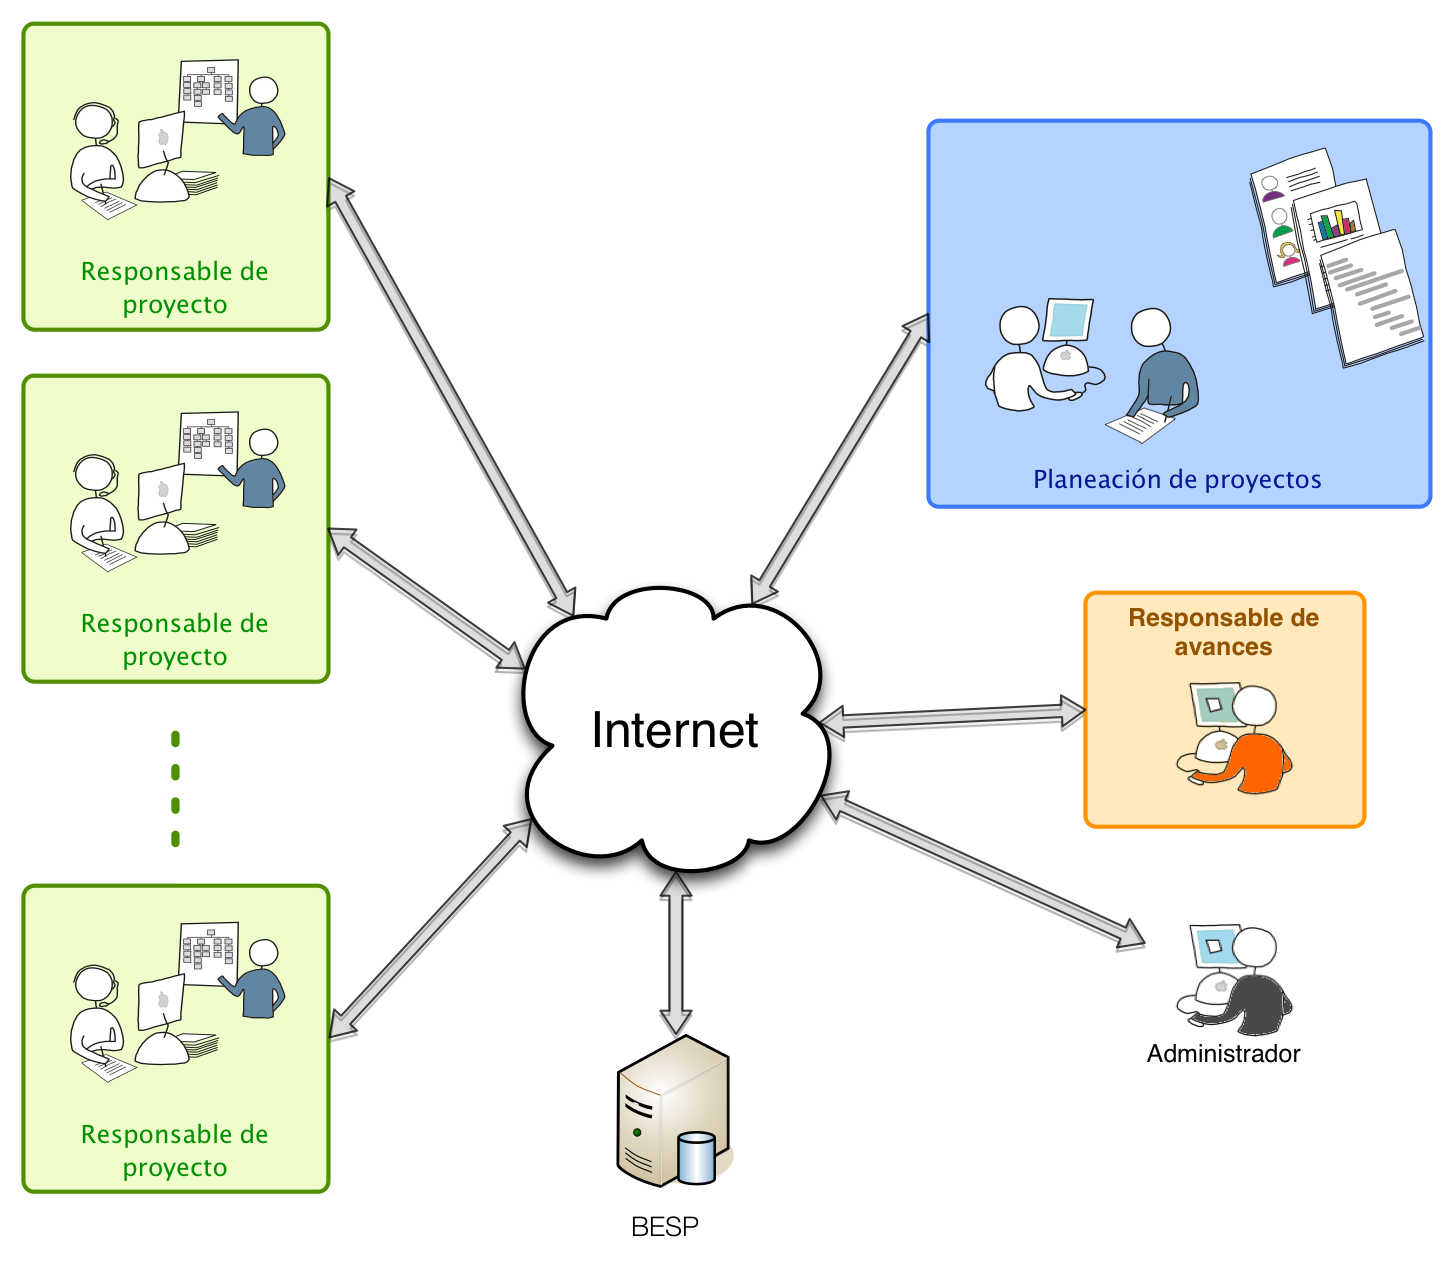
\includegraphics[width=.7\textwidth]{images/arquitectura}}
		\caption{Arquitectura del sistema.}
		\label{fig:arquitectura}
	\end{center}
\end{figure}

En la figura~\ref{fig:arquitectura} se describe la estructura del sistema, en ella se detalla ...



%=========================================================
%=========================================================
\chapter{Planeación del Tiempo}	
\label{cap:tiempo}

	Este capítulo presenta el desglose de la planeación del tiempo del proyecto, contiene la lista de actividades, entregables y esfuerzo requerido para el proyecto, así como las metodologías a utilizar.

%---------------------------------------------------------
\section{Diagrama de Gantt}

\begin{figure}[htbp!]
	\begin{center}
		\fbox{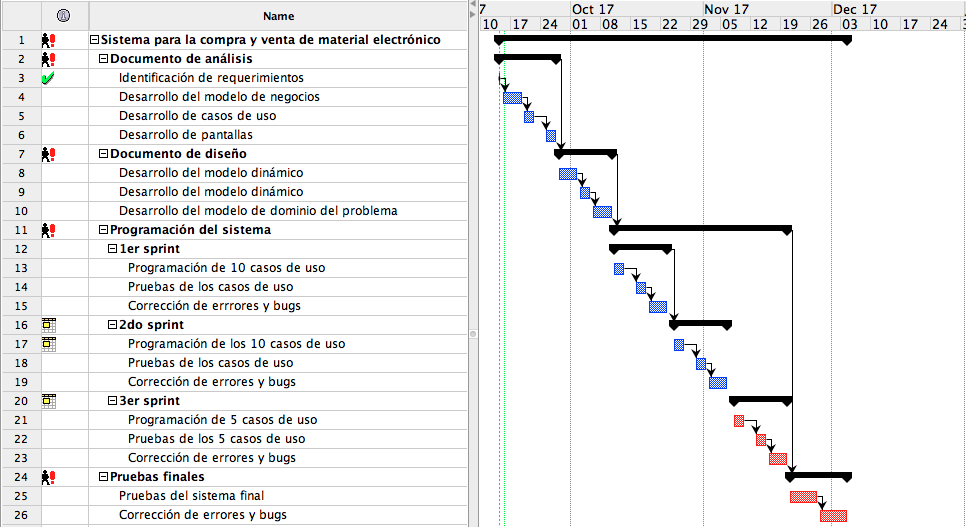
\includegraphics[width=.8\textwidth]{images/plan}}
		\caption{Plan de trabajo del proyecto}
		\label{fig:plan}
	\end{center}
\end{figure}

%---------------------------------------------------------
\section{Entregables}

Los entregables que se tendrán durante el desarrollo del proyecto son los siguientes:

\begin{enumerate}
	\item E2 - Documento de análisis: Miércoles 27 de Septiembre de 2017.
	\item E3 - Documento de diseño: Miércoles 11 de Octubre de 2017.
	\item E4 - Programación de 10 casos de uso y pruebas: Miércoles 25 de Octubre de 2017.
	\item E5 - Programación de 10 casos de uso y pruebas: Miércoles 08 de Nombre de 2017.
	\item E6 - Programación de 5 casos de uso y pruebas: Miércoles 22 de Noviembre de 2017.
	\item E7 - Corrección de errores y sistema final: Miércoles 06 de Diciembre de 2017.
\end{enumerate}



%=========================================================

%=========================================================
\chapter{Planeación de Capital Humano}	
\label{cap:capHumano}

	En este capítulo se presenta la planeación del capital humano del proyecto. Se especifican los integrantes, el organigrama, las habilidades de cada integrante, así como sus roles y responsabilidades en el proyecto.

%---------------------------------------------------------
\section{Organigrama}	

\cdtInstrucciones{
	Arme un diagrama jerárquico que capture la cadena de mando o de  información en el proyecto identificando los principales roles en el equipo de trabajo del proyecto.
}

En la figura~\ref{fig:organigrama} se presentan los roles y la cadena de mando en el proyecto. 

\begin{figure}[htbp]
	\begin{center}
		\fbox{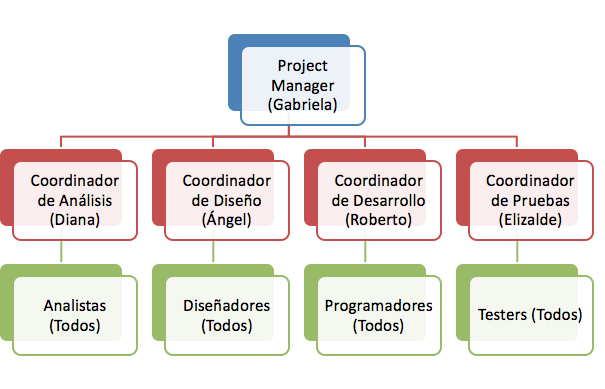
\includegraphics[width=.8\textwidth]{images/Organigrama1}}
		\caption{Organigrama del proyecto}
		\label{fig:organigrama}
	\end{center}
\end{figure}


%---------------------------------------------------------
\section{Responsabilidades}

\cdtInstrucciones{
	Para cada Rol en el proyecto especifique una descripción, responsabilidades dentro del proyecto y habilidades o perfil que se debe cubrir para el puesto.
}


\subsection{Project Manager}
	Líder de proyecto y encargado de el cumplimiento del objetivo del proyecto.
\begin{description}
	\item[Responsabilidades:] \cdtEmpty 	
    \begin{itemize}
    	\item Reconocer los riesgos que puedan impactar la probabilidad de éxito del proyecto.
    	\item Crear políticas para reducir el impacto de los riesgos.
    	\item Planear la ejecución del proyecto en su totalidad.
    	\item Resolver los problemas que se presenten durante la ejecución del proyecto.
    	\item Crear acuerdos entre los coordinadores de las áreas involucradas en el proyecto.
    \end{itemize}
\end{description}

\subsection{Coordinador de Análisis}
	Líder de los analistas y encargado del documento de análisis.
\begin{description}
	\item[Responsabilidades:] \cdtEmpty 	
    \begin{itemize}
    	\item Establecer la forma de trabajo de los analistas y darla a conocer a todo el equipo.
    	\item Asignar tareas a los miembros del equipo de análisis.
    	\item Realizar entrevistas a los usuarios.
    	\item Registrar los tiempos requeridos para realizar las tareas de análisis.
    	\item Realizar el mapeo de procesos.
    	\item Documentar requerimientos.
    	\item Documentar casos de uso.
    	\item Identificar y documentar reglas y términos de negocio.
    	\item Diseñar pantallas.
    	\item Realizar mapas de navegación.
    	\item Responder las dudas en torno al análisis.
    	\item Supervisar el avance del equipo de análisis.
    	\item Establecer acuerdos con el resto de los coordinadores.
    	\item Verificar el trabajo de los analistas.
    	\item Participar en las reuniones de mejora de procesos.
    	\item Documentar lecciones aprendidas.
    \end{itemize}
\end{description}

\subsection{Analista}
	Encargado de realizar el documento de análisis.
\begin{description}
	\item[Responsabilidades:] \cdtEmpty 	
    \begin{itemize}
    	\item Realizar el mapeo de procesos.
    	\item Documentar requerimientos.
    	\item Documentar casos de uso.
    	\item Identificar y documentar reglas y términos de negocio.
    	\item Diseñar pantallas.
    	\item Realizar mapas de navegación.
    	\item Notificar avance al Coordinador de Análisis.
    	\item Notificar cualquier cambio al alcance al Coordinador de Análisis.
    	\item Documentar lecciones aprendidas.
    	\item Participar en las reuniones de mejoras de procesos.
    \end{itemize}
\end{description}

\subsection{Coordinador de diseño}
	Líder de los diseñadores y encargado del documento de diseño.
\begin{description}
	\item[Responsabilidades:] \cdtEmpty 	
    \begin{itemize}
    	\item Establecer la forma de trabajo de los diseñadores y darla a conocer a todo el equipo.
    	\item Planear las actividades de la etapa de diseño.
    	\item Asignar tareas a los miembros del equipo de diseño.
    	\item Traducir los elementos de análisis a en clases y entidades.
    	\item Realizar los diagramas de secuencia para los procesos del sistema.
    	\item Generar el diagrama entidad-relación de la base de datos.
    	\item Responder las dudas en torno al diseño del sistema.
    	\item Supervisar el avance del equipo de diseño.
    	\item Establecer acuerdos con el resto de los coordinadores.
    	\item Verificar el trabajo de los diseñadores.
    	\item Apoyar al arquitecto de software en la definición de la infraestructura.
    	\item Participar en las reuniones de mejora de procesos.
    	\item Registrar los tiempos requeridos para realizar las tareas de diseño.
    	\item Documentar lecciones aprendidas.
    \end{itemize}
\end{description}

\subsection{Diseñador}
	Encargado de realizar el documento de diseño.
\begin{description}
	\item[Responsabilidades:] \cdtEmpty 	
    \begin{itemize}
    	\item Traducir los elementos de análisis en clases y entidades.
    	\item Generar el diagrama entidad-relación de la base de datos.
    	\item Realizar los diagramas de secuencia para los procesos del sistema.
    	\item Informar al Coordinador de Diseño sobre posibles cambios o problemas en la arquitectura del sistema.
    	\item Notificar al Coordinador de Diseño el avance.
    	\item Participar en las reuniones de mejoras de procesos.
    	\item Documentar lecciones aprendidas.
    \end{itemize}
\end{description}

\subsection{Coordinador de desarrollo}
	Líder de los desarrolladores y encargado de la programación del sistema de acuerdo al documento de análisis y diseño.
\begin{description}
	\item[Responsabilidades:] \cdtEmpty 	
    \begin{itemize}
    	\item Establecer la forma de trabajo de los programadores y darla a conocer a todo el equipo.
    	\item Planear las actividades de la etapa de implementación.
    	\item Asignar tareas a los miembros del equipo de desarrollo.
    	\item Implementar los componentes necesarios para los casos de uso asignados, definidos en el diseño.
    	\item Realizar pruebas funcionales sobre los elementos programados.
    	\item Aplicar las buenas prácticas de programación definidas para el proyecto.
    	\item Asegurar la integración de los módulos del sistema.
    	\item Responder las dudas en torno a la programación del sistema.
    	\item Supervisar el avance del equipo de desarrollo.
    	\item Establecer acuerdos con el resto de los coordinadores.
    	\item Verificar el trabajo de los programadores.
    	\item Apoyar al arquitecto de software en la definición de la infraestructura.
    	\item Participar en las reuniones de mejora de procesos.
    	\item Definir la forma de solucionar las incidencias reportadas en la programación.
    	\item Registrar los tiempos requeridos para realizar las tareas de desarrollo.
    	\item Documentar lecciones aprendidas.
    \end{itemize}
\end{description}

\subsection{Programador}
	Encargado de programar el sistema acorde a la documentación.
\begin{description}
	\item[Responsabilidades:] \cdtEmpty 	
    \begin{itemize}
    	\item Implementar los componentes necesarios para los casos de uso asignados, definidos en el diseño.
    	\item Realizar pruebas funcionales sobre los elementos programados.
    	\item Aplicar las buenas prácticas de programación definidas para el proyecto.
    	\item Asegurar la integración de los módulos del sistema.
    	\item Notificar el avance al Coordinador de Programación.
    	\item Participar en las reuniones de mejoras de procesos.
    	\item Documentar lecciones aprendidas.
    \end{itemize}
\end{description}

\subsection{Coordinador de pruebas}
	Líder de los testers y encargado de asegurarse de que el sistema funcione como se estableció en la documentación, y de corrección de errores y bugs.
\begin{description}
	\item[Responsabilidades:] \cdtEmpty 	
    \begin{itemize}
    	\item Establecer la forma de trabajo de los testers y darla a conocer a todo el equipo.
    	\item Planear las actividades de la etapa de pruebas.
    	\item Asignar tareas a los miembros del equipo de pruebas.
    	\item Identificar los escenarios a probar en un caso de uso, módulo o sistema.
    	\item Documentar los guiones de prueba del sistema.
    	\item Documentar los datos de prueba.
    	\item Generar los scripts de prueba para cada escenario.
    	\item Ejecutar las pruebas y documentar los resultados.
    	\item Dar retroalimentación a los programadores sobre los resultados.
    	\item Dar seguimiento a las incidencias encontradas.
    	\item Responder las dudas en torno a las pruebas e incidencias encontradas dentro del sistema.
    	\item Supervisar el avance del equipo de pruebas.
    	\item Supervisar que el proceso de pruebas se realice correctamente.
    	\item Establecer acuerdos con el resto de los coordinadores.
    	\item Verificar el trabajo de los testers.
    	\item Participar en las reuniones de mejora de procesos.
    	\item Registrar los tiempos requeridos para realizar las tareas de pruebas.
    	\item Documentar lecciones aprendidas.
    \end{itemize}
\end{description}

\subsection{Tester}
	Encargado de probar el sistema y reportar el estado de las funciones de éste.
\begin{description}
	\item[Responsabilidades:] \cdtEmpty 	
    \begin{itemize}
    	\item Identificar los escenarios a probar en un caso de uso, módulo o sistema.
    	\item Documentar los guiones de prueba del sistema.
    	\item Documentar los datos de prueba.
    	\item Generar los scripts de prueba para cada escenario.
    	\item Ejecutar las pruebas y documentar los resultados.
    	\item Dar retroalimentación a los programadores sobre los resultados.
    	\item Dar seguimiento a las incidencias encontradas.
    	\item Notificar el avance al Coordinador de Pruebas.
    	\item Notificar al Coordinador de Pruebas de posibles fallos en el análisis o implementación.
    	\item Participar en las reuniones de mejoras de procesos.
    	\item Documentar lecciones aprendidas.
    \end{itemize}
\end{description}

%---------------------------------------------------------
\section{Staff}

\cdtInstrucciones{
	Liste a los integrantes del proyecto especificando su rol, y datos de contacto.\\
}

\begin{table}[hbtp!]
    \noindent\begin{tabular}{|p{.25\textwidth}|p{.15\textwidth}|p{.15\textwidth}|p{.35\textwidth}|}
    	\hline
    	{\bf Nombre} & {\bf Rol} & {\bf Teléfonos} & {\bf Correo}\\
    	\hline
	Moreno González Gabriela & Project Manager & 55 7488 9938 & gonzalez\_gabriela12@hotmail.com \\
        	\hline
    	Mejía Mendoza Diana Laura & Coordinadora de análisis & 55 2034 4711 & dianal\_mm9@hotmail.com \\
    	\hline
	Ferreira Osorno Ángel & Coordinador de diseño & 55 6182 2900 & isc.angel.ipn@gmail.com \\
	\hline
	Mendoza Saavedra Roberto & Coordinador de desarrollo & 55 2184 2095 & isc.robertomendoza@gmail.com \\
	\hline
	Corona Luis Ángel & Coordinador de pruebas & 55 1512 1615 & eli17escom@gmail.com \\
    \end{tabular}
	\caption{Integrantes del proyecto.}
	\label{tbl:staff}
\end{table}



%=========================================================
%=========================================================
\chapter{Planeación de la Comunicación}
\label{cap:comunicacion}	

\cdtInstrucciones{Una vez que haya identificado las necesidades de comunicación en el proyecto y acordado la forma de comunicación interna especifique: información identificada, quien la necesita, quien la genera y canal de comunicación.\\}

\begin{table}[hbtp!]
    \noindent\begin{tabular}{|p{.25\textwidth}|p{.15\textwidth}|p{.2\textwidth}|p{.3\textwidth}|}
    	\hline
    	{\bf Información} & {\bf Responsable} & {\bf Receptor} & {\bf Canal de comunicación}\\
    	\hline
    	Requerimientos actualizados & Analista &
    \begin{Titemize}
    	\Titem  Diseñadores 
    	\Titem Programadores
    	\Titem Project Manager
    \end{Titemize}
     & Estarán disponibles en el repositorio \url{https://github.com/HilaArtzunari/Sworkware}\\
    	\hline	 
    	Diagrama de casos de uso & Analista & 
	 \begin{Titemize}
    		\Titem  Diseñadores 
    		\Titem Programadores
    		\Titem Project Manager
    	\end{Titemize} 
     & Estarán disponibles en el repositorio \url{https://github.com/HilaArtzunari/Sworkware}\\
    	\hline
	Diagramas de secuencia & Diseñador & 
	 \begin{Titemize}
    		\Titem Programadores
    		\Titem Project Manager
    	\end{Titemize} 
     & Estarán disponibles en el repositorio \url{https://github.com/HilaArtzunari/Sworkware}\\
     	\hline
	Base de datos & Diseñador & 
	 \begin{Titemize} 
    		\Titem Programadores
    		\Titem Project Manager
    	\end{Titemize} 
     & Estarán disponibles en el repositorio \url{https://github.com/HilaArtzunari/Sworkware}\\
     	\hline
	Programación de casos de uso & Programador & 
	 \begin{Titemize} 
    		\Titem Testers
    		\Titem Project Manager
    	\end{Titemize}
     & Estarán disponibles en el repositorio \url{https://github.com/HilaArtzunari/Sworkware}\\
     	\hline
	Testeo de casos de uso & Tester & 
	 \begin{Titemize} 
    		\Titem Analistas
		\Titem Diseñadores
    		\Titem Project Manager
    	\end{Titemize} 
     & Estarán disponibles en el repositorio \url{https://github.com/HilaArtzunari/Sworkware}\\
    \end{tabular}
	\caption{Plan de comunicación interna.}
	\label{tbl:planComunicacionInt}
\end{table}



%==========================================================
\clossing
\end{document}
